% \section{Long-term (1985 – 2018) monitoring of forest cover changes in the Atlantic Forest using Landtrendr algorithm}
\section{Monitoramento de longo prazo (1985 – 2018) das mudanças florestais na Mata Atlântica utilizando o algoritmo Landtrendr}
\subsection{Introdução}
\hspace{13pt} Introdução.

\subsection{Materiais e Métodos}
\subsubsection{Área de estudo}
\hspace{13pt} O estudo abrange toda a área do bioma da Mata Atlântica brasileira (Figura \ref{fig:mata_atlantica}), que possui atualmente uma área total de aproximadamente 1.1 Mkm2 ou 110 Mha. O bioma está presente em 15 estados brasileiros e é onde se localiza grande parte da atividade econômica e população do pais. Atualmente, vivem na Mata Atlântica cerca de 72\% da população brasileira, o que em parte explica o fato de hoje apenas cerca de 12\% de sua cobertura natural ter persistido.. O bioma ainda possui 75,6\% das espécies ameaçadas e endêmicas do Brasil, o que o torna um dos mais prioritários para conservação no país. Além disso, estima-se que entre 43\% e 45\% do total de espécies de plantas e vertebrados sejam restritas a esse bioma \citep{scarano2014}.

\begin{figure}[h!]
    \centering
    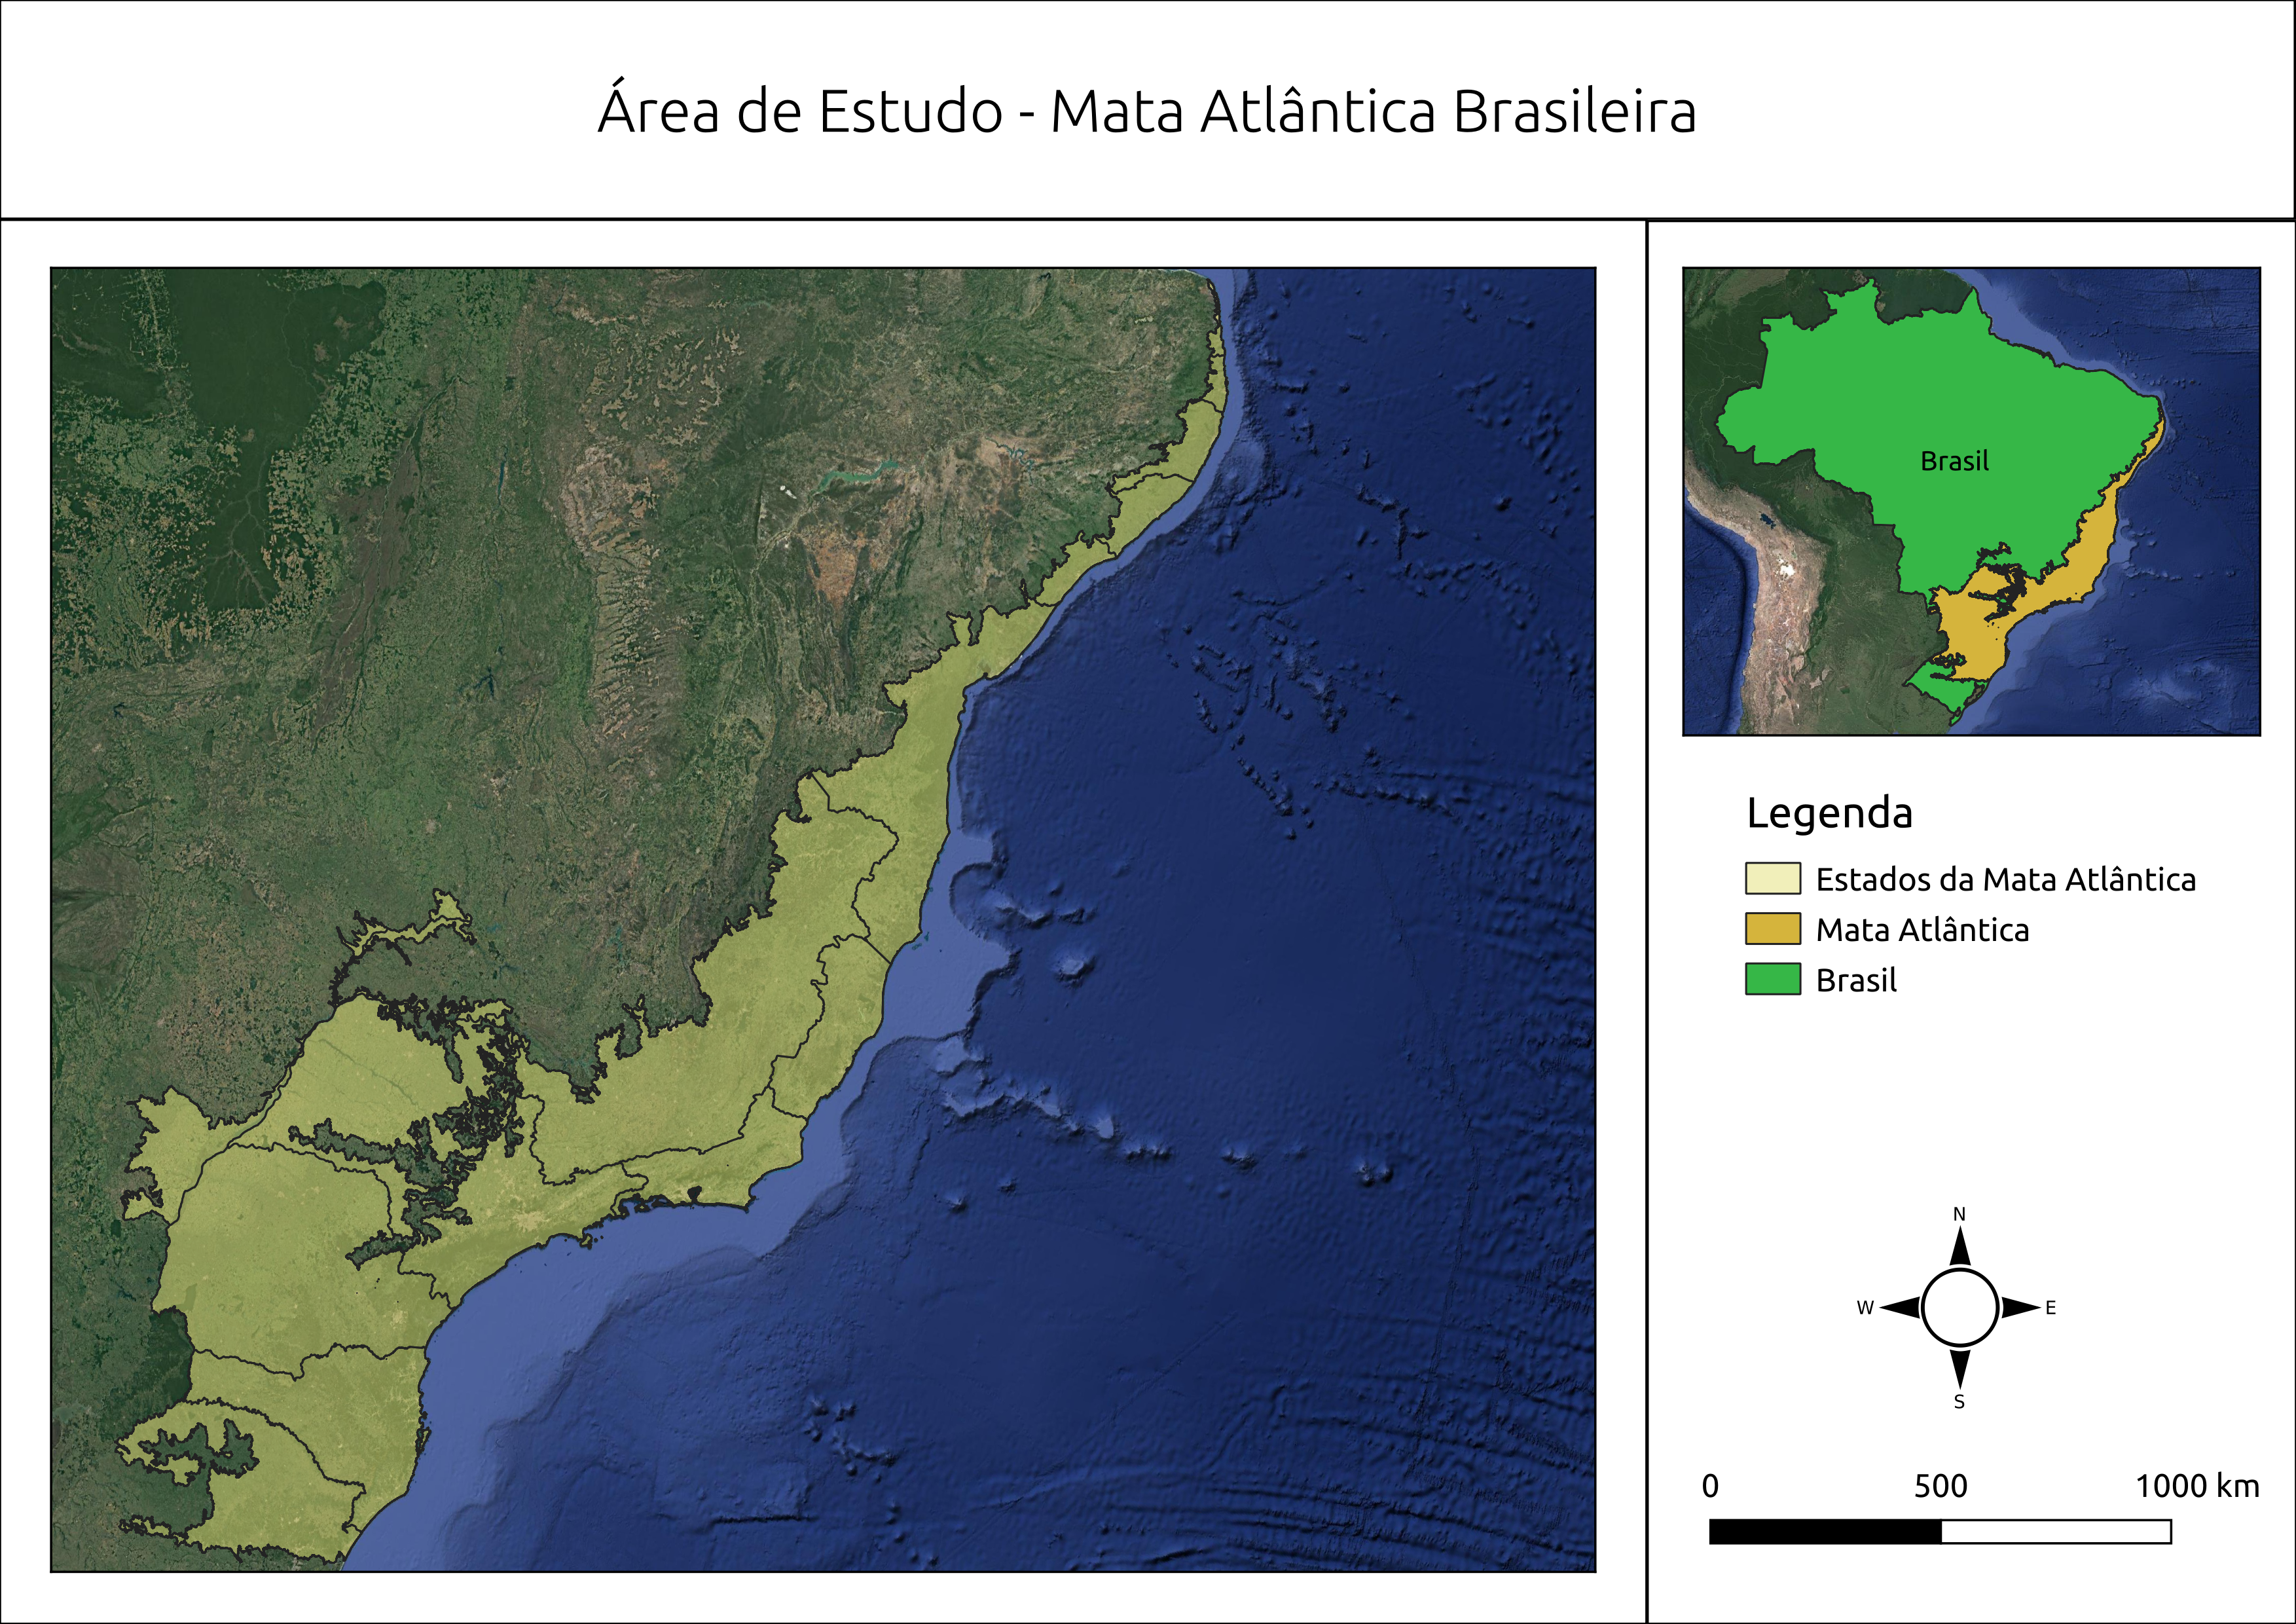
\includegraphics[scale=.5]{images/mata_atlantica_thin.png}
    \caption{Área de Estudo - Mata Atlântica brasileira}
    \label{fig:mata_atlantica}
\end{figure}

Na época da chegada dos portugueses no Brasil, a Mata Atlântica cobria cerca de 1,5 milhões de quilômetros quadrados, estendendo-se ao longo de 3 mil quilômetros da costa brasileira - do Rio Grande do Sul ao Rio Grande do Norte - e penetrando pelo interior, cruzando São Paulo, Minas Gerais e Mato Grosso do Sul até as fronteiras da Argentina e do Paraguai \citep{scarano2014}. Cerca de 500 anos depois, esse extenso e representativo bioma abriga mais de 100 milhões de pessoas, cerca de 1/4 das quais ainda vivem na pobreza \citep{scarano2014}.

Segundo o projeto Mapbiomas, a área total de florestas no bioma em 1985 era de X e em 2018 de X. Já a área de florestas que não sofreram mudanças significativas (pseudo-invariantes) durante o período de 1985 até 2018 foi de aproximadamente 21.4 Mha. Deste total, somente  30\% da vegetação nativa remanescente está protegida legalmente através de unidades de conservação.

% Apesar dos importantes avanços obtidos nesta agenda na última década – como a restauração de aproximadamente 1,4 milhões de hectares entre 2011 e 2020 – muito ainda precisa ser feito \citep{CROUZEILLES2019}

\subsubsection{Dados de entrada}
\hspace{13pt} Para o mapeamento do bioma consideramos um intervalo anual que compreendeu todos os anos de 1985 até 2018 utilizando imagens do satélite Landsat das séries 5, 7 e 8. A escolha desse período de análise se deu por conta do início da captura de dados iniciado em 1 de março de 1984 pelo satélite Landsat 5 e consequente disponibilidade de dados pela comunidade científica para o mesmo período, o que facilitou a verificação e validação dos resultados. Para cobrir todos os 110 Mha do bioma foi necessário a compilação e processamento de 88 cenas Landsat, cada uma com cerca de 23 imagens com por ano, o que dá algo em torno de 67 mil imagens. Se considerarmos que cada uma dessas imagens possui pelo menos 7 bandas, chegamos a um cubo multidimensional de quase meio milhão de bandas. Um processamento que sem dúvidas só seria possível com o advento das tecnologias já citadas.

Todas as imagens utilizadas são da coleção \emph{surface reflectance}, o que significa que já possuem correção geométrica, radiométrica e possuem valor físico referente a superfície terrestre. Além disso, as imagens passaram por processo de harmonização para evitar acúmulo de ruídos. As séries temporais foram criadas utilizando uma função própria do Landtrendr.

\subsubsection{Método de análise}
\hspace{13pt} A análise das trajetórias foi feita utilizando o algoritmo Landtrendr em sua versão para a plataforma Google Earth Engine (GEE) \citep{Kennedy2018}. As vantagens da implementação do algoritmo no GEE em relação a sua versão original em ENVI/IDL está na possibilidade de sua aplicação em áreas extensas. Além disso, a versão para GEE elimina grande parte dos desafios técnicos presentes em sua implementação clássica. No entanto, apesar do ganho significativo no tempo de processamento quando comparado a sua versão em IDL, o Landtrendr GEE também apresenta algumas limitações. Uma das maiores está na limitação na extensão da análise para apenas uma imagem Landsat por vez. A plataforma apresentou erros sistemáticos quando foi requisitada para processar análises para toda a Mata Atlântica de uma só vez, por exemplo. Com isso, o processamento teve de ser feito em etapas. 

Com isso, as etapas tiveram de ser divididas por cenas Landsat, neste caso, 88 cenas (Figura \ref{fig:pathrow_centroids}). Como o resultado do algoritmo é dado de forma separada por cena, foi necessário juntar todas as camadas geradas em uma única após uma etapa extra de pós-processamento. Devido a ruídos presentes nas bordas das imagens Landsat e a sobreposição natural entre imagens diferentes, nem todos os pixels presentes nas bordas apresentaram resultados similares. Juntar todos as 88 camadas de resultados em uma se tornou um desafio e só foi possível através criação de polígonos de voronoi \citep{Okabe}, o que possibilitou utilizarmos somente as áreas mais próximas do centro das camadas geradas pelo algoritmo. 

\begin{figure}[h!]
    \centering
    \includegraphics[scale=.5]{images/ma_pathrow_centroids.png}
    \caption{Pathrows das imagens Landasat e seus respectivos centróides que foram utilizados para delimitar as cenas a serem processadas pelo algoritmo}
    \label{fig:pathrow_centroids}
\end{figure}

Os polígonos de voronoi foram gerados através da extração dos centroides dos polígonos delimitadores das cenas Landsat e posteriormente utilizados para a criação dos polígonos com as áreas centrais (Figura \ref{fig:voronoi_ma}). Após a geração dos polígonos de voronoi, o mesmos foram utilizados para recordar os resultados de forma a limpar possíveis sobreposições. Após o recorte, todas as imagens foram agregadas para toda extensão do bioma e separadas banda a banda para análise posterior.

\begin{figure}[H]
    \centering
    \includegraphics[scale=.5]{images/voronoi_mata_atlantica.png}
    \caption{Diagrama de Voronoi criado a partir dos centróides.}
    \label{fig:voronoi_ma}
\end{figure}

Tanto resultados para o cenário de perda quanto de ganho foram gerados com o objetivo de detectar supressões e processos de degradação como também de restauração e regeneração da floresta. Para este estudo, o Landtrendr foi aplicado utilizando todos seus parâmetros padrões. O tipo de eventos (perda ou ganho) foram organizados de acordo com seu maior evento (\textit{Greatest Loss / Greatest Gain}).

Toda a etapa de pós-processamento dos dados gerados pelo Landtrendr no GEE foi desenvolvida em ambiente \textit{offline} utilizando ferramentas \textit{open source} como o QGIS \citep{QGIS_software}, GDAL \citep{gdal}, e a linguagem de programação R \citep{Rsoftware} utilizando os pacotes Raster \citep{raster}, Terra \cite{terra}, gdalUtils \citep{gdalutils} e o MLR \citep{mlr}.

\subsubsection{Processamento dos cenários de ganho}
\hspace{13pt} Para o cenário de ganho, todos os parâmetros padrão do algoritmo foram mantidos sem nenhum tipo de restrição. Cenários de magnitude (\textit{magnitude}), valor prévio (\textit{previous value}), ano de detecção (\textit{year of detection}), duração (\textit{duration}) e taxa (\textit{rate}) forma gerados e posteriormente pós-processados para limpeza de ruídos ou para retirada de valores indesejados. 

Primeiramente, foi gerado uma máscara com todas as áreas pseudo-invariantes entre os anos da análise (1985 - 2018) com o intuito de limpar detecções de mudança muito pequenas. Além disso, foram mascarados todos os eventos com duração menor ou igual a 4 anos, já que não gostaríamos de incorporar eventos ainda muito recentes que poderiam ser identificados como falsos eventos de mudança. O valor mínimo de 5 anos para eventos de ganho ajuda a identificar apenas eventos mais longos que tiveram tempo de apresentar respostas espectrais significativas de recuperação. Com 5 anos a vegetação já passa a apresentar um estágio sucessional característico de floresta secundária inicial \citep{Chazdon2014}. 

\subsubsection{Processamento dos cenários de perda}
\hspace{13pt} Assim como o cenário de ganho, o processamento do cenário de perda utilizou todos os parâmetros padrões do algoritmo sem nenhum tipo de restrição com o objetivo de realizar limpezas nos resultados obtidos apenas em uma etapa de pós-processamento. Os mesmos cenários de magnitude (\textit{magnitude}), valor prévio (\textit{previous value}), ano de detecção (\textit{year of detection}), duração (\textit{duration}) e taxa (\textit{rate}) forma gerados.

No caso das perdas, criou-se uma máscara para garantir que o Landtrendr fosse capaz de detecção mudanças de perda apenas em áreas que foram classificadas como floresta pelo projeto Mapbiomas no ano de 1985. Essa máscara ajuda na não seleção de áreas que nem mesmo eram classificadas como florestas mas que sofreram algum tipo de perda com magnitude grande o suficiente para ser detectada pelo algoritmo. Além disso, uma outra máscara foi gerada, para excluir áreas que apesar de terem sido mapeadas em 1985 como floresta e terem sofrido algum tipo de perda significativa, sofreram algum processo de restauração ou regeneração natural ao longo dos anos. Sendo assim, o resultado final para o dado de perdas visou somente a seleção de áreas que tiveram floresta, que perderam essa vegetação e que não apresentaram nenhum processo de recuperação significativa.

Diferentemente dos dados de ganho, os dados de perda tem como característica importante a grande variabilidade na duração dos eventos. Sendo assim, utilizou-se a camada de duração para gerar, além das camadas de perda gerais, camadas de perda com duração igual a um ano e camadas com duração superior à um ano. Esta diferenciação é importante para que possamos identificar eventos de perda rápida, sejam eles de natureza antrópica ou natural, normalmente associados à cortes rasos ou queimadas. 

% \subsubsection{Validação}

\subsection{Resultados e Discussões}

\subsubsection{Os eventos de perda na Mata Atlântica}

\begin{figure}[H]
    \centering
    \includegraphics[scale=.5]{images/heatmap_loss_masked85_maskedgain.png}
    \caption{Todos os eventos de perda na Mata Atlântica entre 1985 e 2018.}
    \label{fig:heat_loss_masked85_maskedgain}
\end{figure}

\begin{figure}[H]
    \centering
    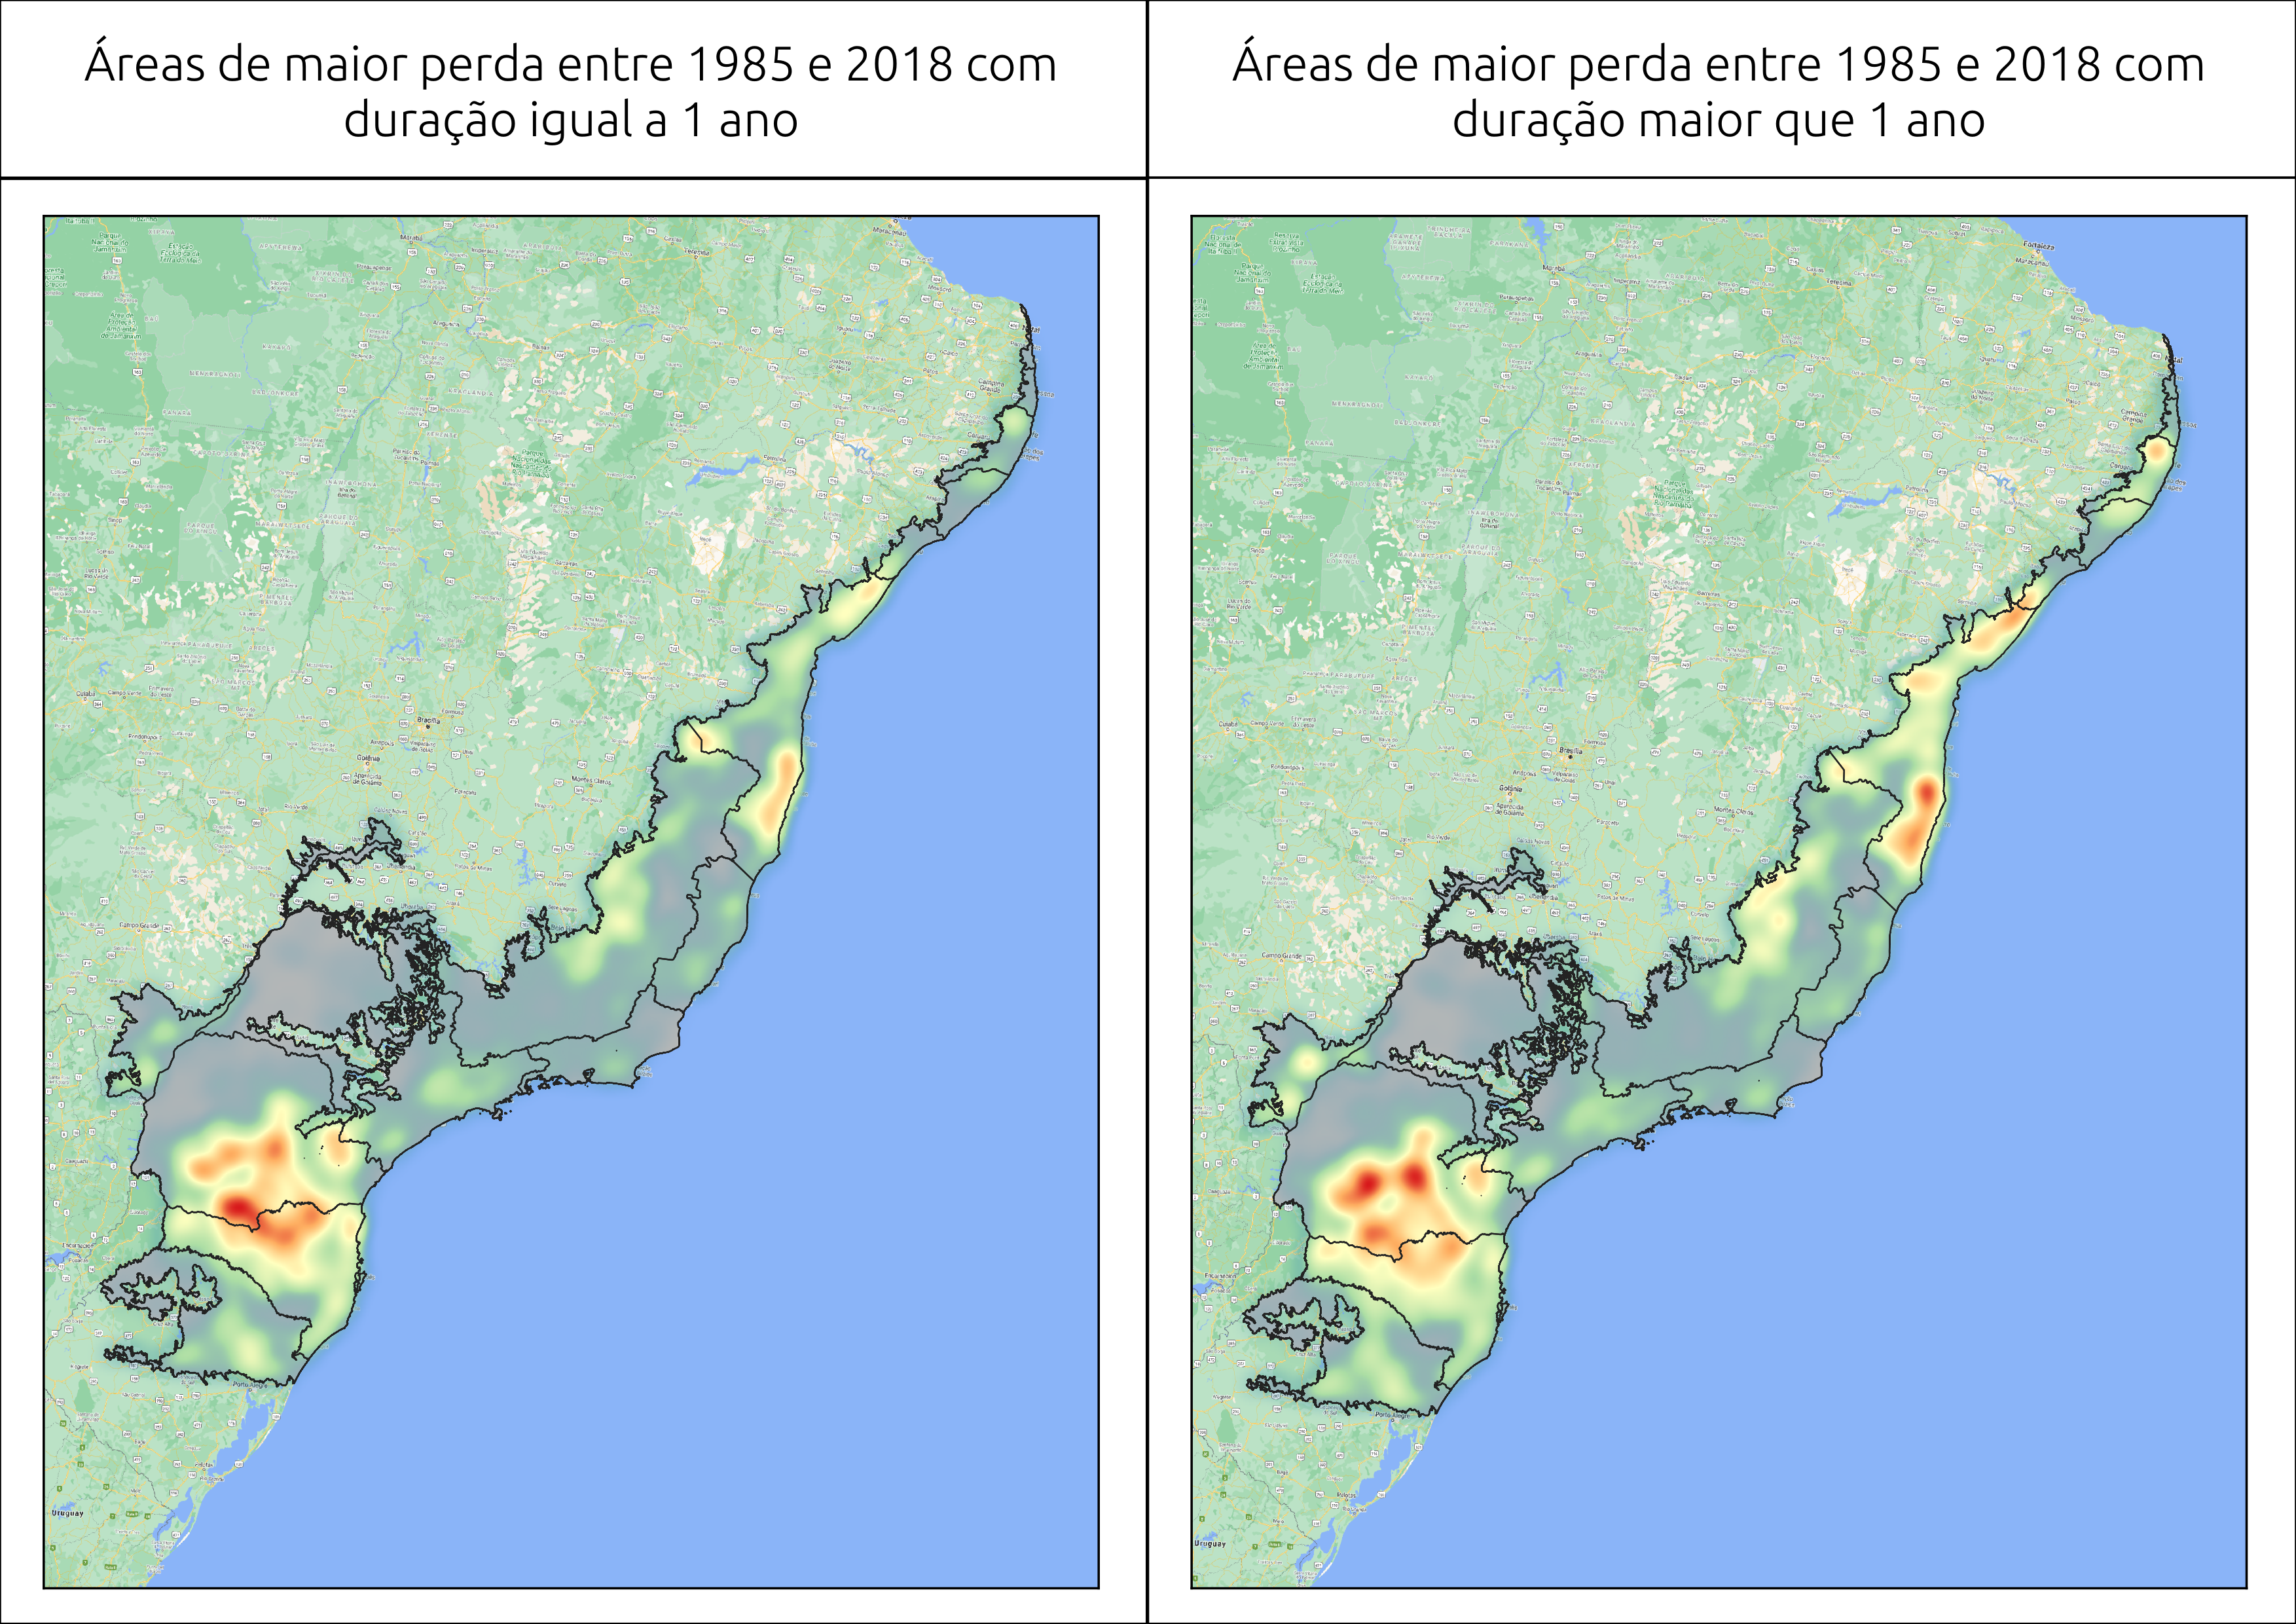
\includegraphics[scale=.5]{images/heatmap_loss_eq1_neq1.png}
    \caption{Mapas com os eventos de perda entre 1985 e 2018 tanto com duração igual a 1 quanto somente maiores que 1.}
    \label{fig:heat_loss_eq1_neq1}
\end{figure}

\subsubsection{Os eventos de ganho na Mata Atlântica}
\subsubsection{A idade das florestas secundárias da Mata Atlântica}

\subsection{Conclusões}